\subsection{Translational Controller}

\begin{frame}{Control Solution}{Translational Controller}
  \begin{figure}[H]
      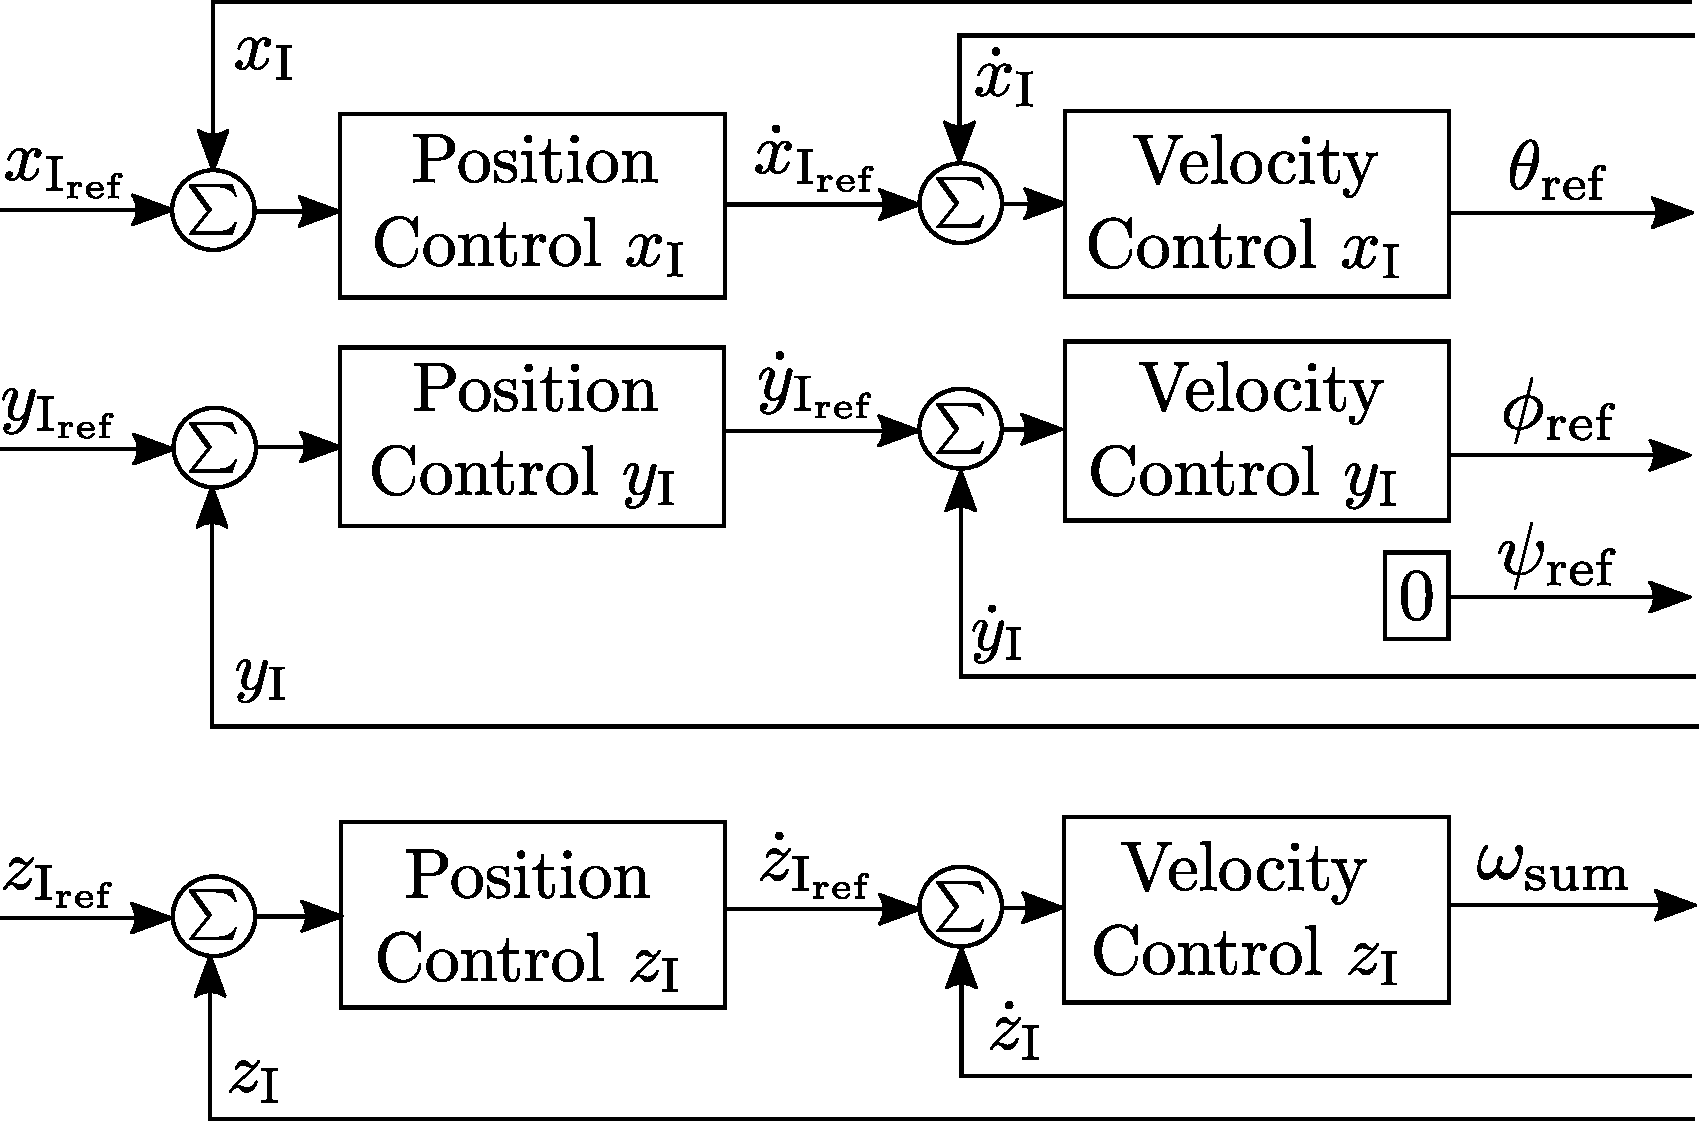
\includegraphics[width=.8\textwidth]{figures/TranslationalControlDiagramSmall}
  \end{figure}      
\end{frame}

\begin{frame}{Control Solution}{Translational Controller}

  \only<1| handout:1>
  {
    \begin{figure}[H]
      \hspace*{-.8cm}
      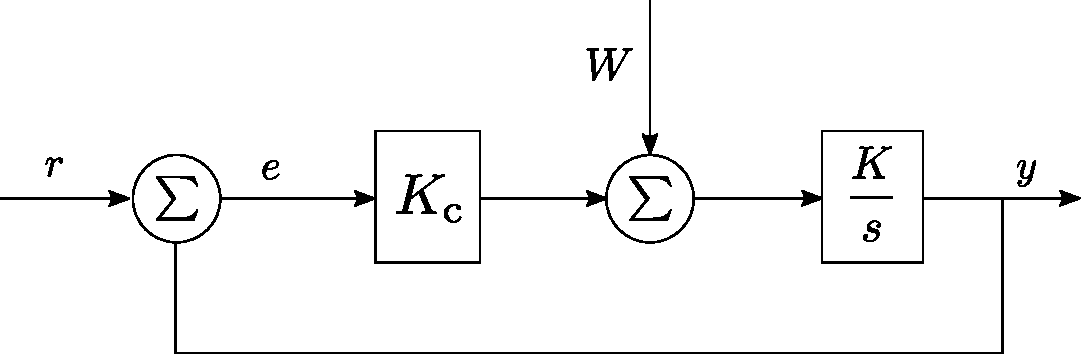
\includegraphics[width=.5\textwidth]{figures/disturbanceP}
    \end{figure}
    \vspace*{1.72cm}
  }

  \only<2| handout:2>
  {
    \begin{figure}[H]
      \hspace*{-.8cm}
      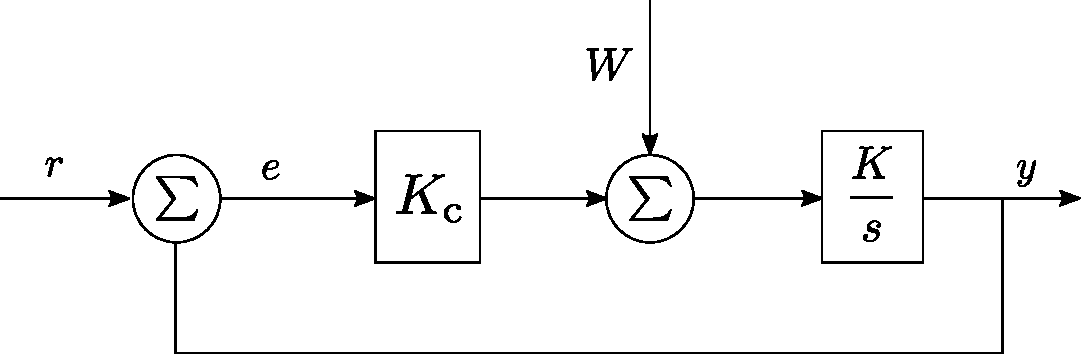
\includegraphics[width=.5\textwidth]{figures/disturbanceP}
    \end{figure}
    \vspace*{.5cm}
    \[
      \frac{y}{W}=\frac{\frac{K}{s}}{1+K_c \frac{K}{s}}=\frac{K}{s+K_c K}
      \Rightarrow \lim_{s \to 0} \frac{K}{s+K_c K} = \frac{1}{K_c}
    \]
  }
  
  \only<3| handout:3>
  {
    \begin{figure}[H]
      \hspace*{-.8cm}
      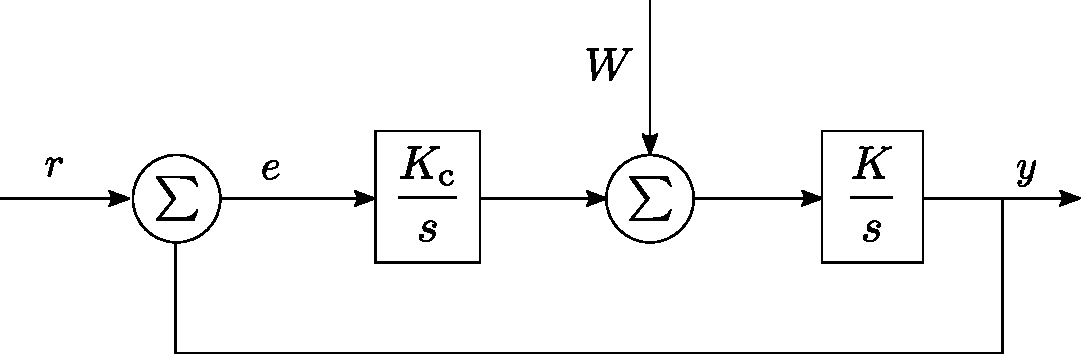
\includegraphics[width=.5\textwidth]{figures/disturbancePI}
    \end{figure}
    \vspace*{.5cm}
    \[
      \frac{y}{W}=\frac{\frac{K}{s}}{1+K_c \frac{K}{s}}=\frac{K}{s+K_c K}
      \Rightarrow \lim_{s \to 0} \frac{K}{s+K_c K} = \frac{1}{K_c}
    \]
  }

  \only<4| handout:4>
  {
    \begin{figure}[H]
      \hspace*{-.8cm}
      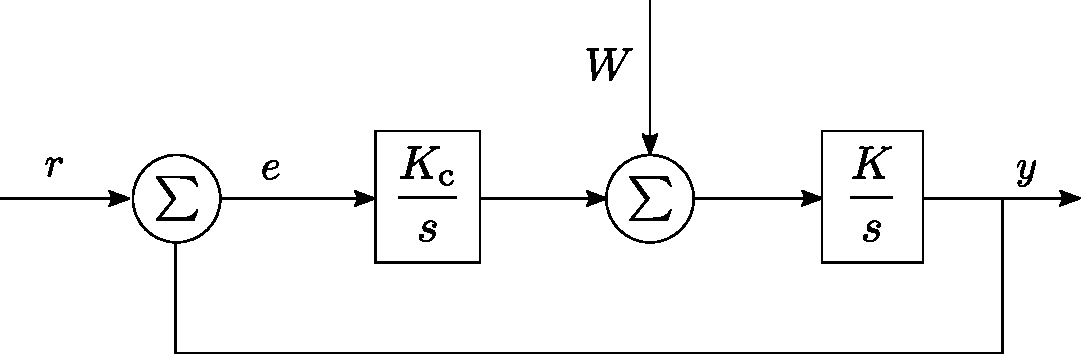
\includegraphics[width=.5\textwidth]{figures/disturbancePI}
    \end{figure}
    \vspace*{.5cm}
    \[\hspace{-.35cm}
      \frac{y}{W}=\frac{\frac{K}{s}}{1+\frac{K_c}{s} \frac{K}{s}} = \frac{Ks}{s^2+K_c K}
      \Rightarrow \lim_{s \to 0} \frac{Ks}{s^2+K_c K} = 0
    \]
  }

\end{frame}

\begin{frame}{Control Solution}{Translational Controller}
  \vspace*{1cm}
  \Large
  \centering{
    $\frac{\dot{x}_\mathrm{I}}{\theta} = \frac{-k_\mathrm{th} 4 \overline{\omega}}{m s}$ \hspace*{1cm}
    $\frac{\dot{y}_\mathrm{I}}{\phi} = \frac{k_\mathrm{th} 4 \overline{\omega}}{m s}$ \hspace*{1cm}
    $\frac{\dot{z}_\mathrm{I}}{\omega_\mathrm{sum}} = \frac{-2 k_\mathrm{th} \overline{\omega}}{m s}$
  }
  \normalsize
  \pause
  \vspace*{1cm}
  \begin{figure}[H]
    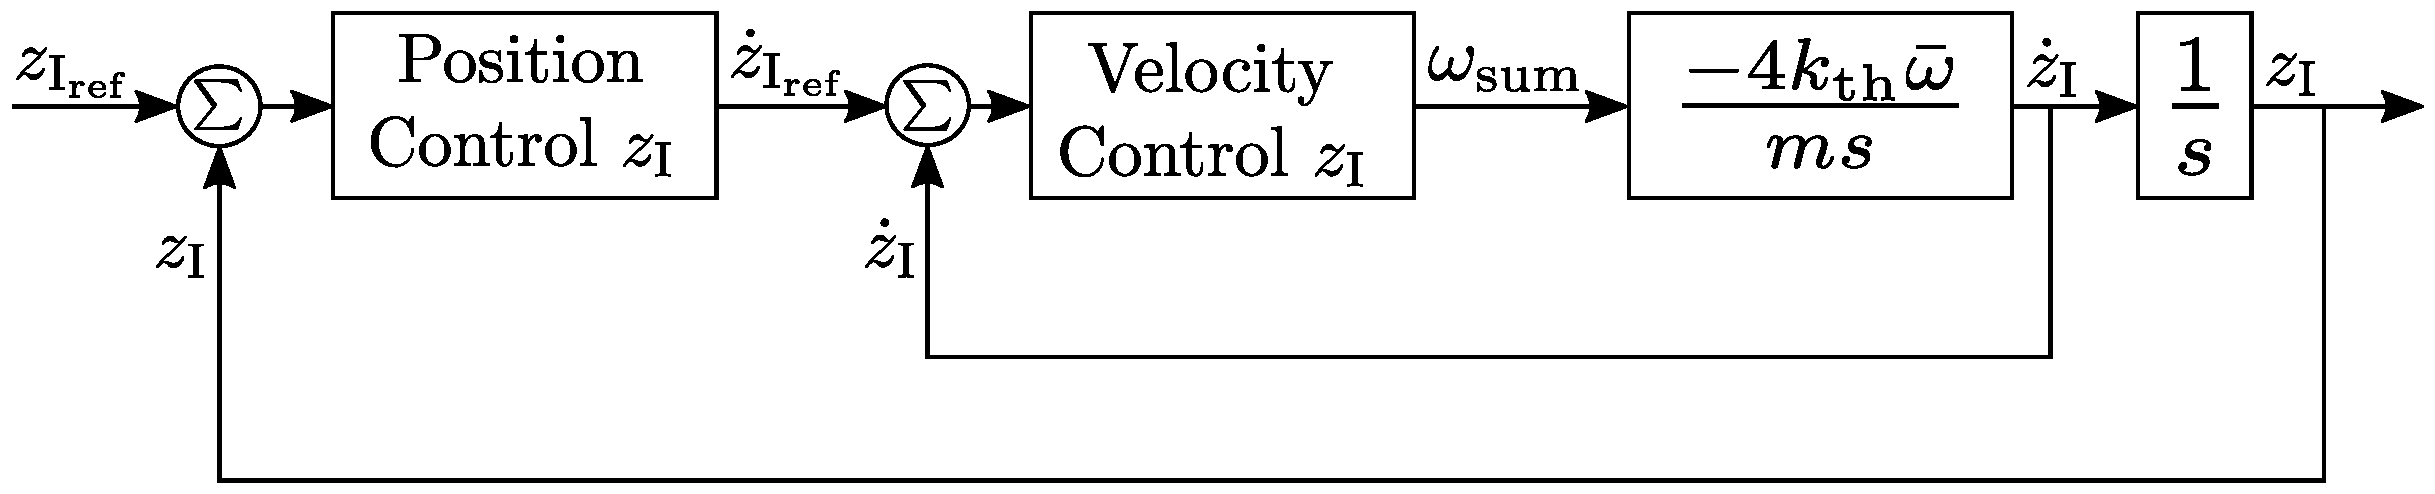
\includegraphics[width=1\linewidth]{figures/TranslationalControlZ}
  \end{figure}
\end{frame}

\begin{frame}{Control Solution}{Translational Controller}
  put three root locus      
\end{frame}

\begin{frame}{Control Solution}{Translational Controller}
  consideration of bandwidth
  equations for velocity controllers
  equations for position controllers
\end{frame}


%%%%%%%%%%%%%%%%
\section{Implementation}
\begin{frame}{Implementation}{}
  FreeRTOS, tasks
\end{frame}

\begin{frame}{Implementation}{Schedule}
  \begin{figure}[H]
    \hspace*{-.8cm}
    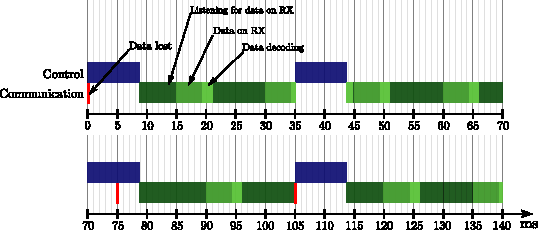
\includegraphics[width=1.1\linewidth]{figures/timingDiagram}
  \end{figure}  
\end{frame}

\begin{frame}{Implementation}{Schedule}
  \begin{figure}[H]
    \hspace*{-.8cm}
    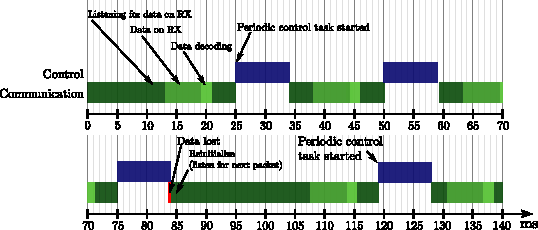
\includegraphics[width=1.1\linewidth]{figures/newTimingDiagram}
  \end{figure}
\end{frame}

\begin{frame}{Implementation}{Schedule}
\hspace*{-.1cm}
  \begin{minipage}{0.49\linewidth}
    \begin{figure}[H]
      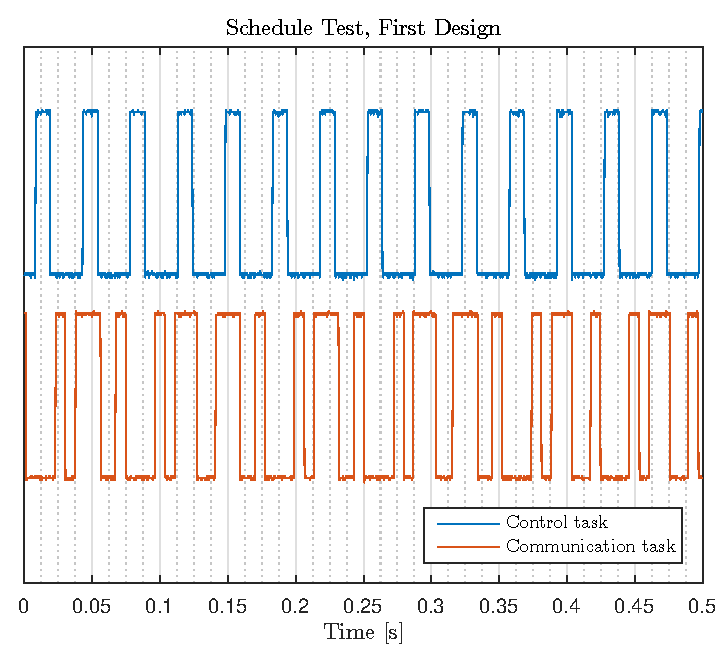
\includegraphics[width=1\linewidth]{figures/scheduleTest}
    \end{figure}
  \end{minipage}\hspace*{.2cm}
  \begin{minipage}{0.49\linewidth}
    \begin{figure}[H]
      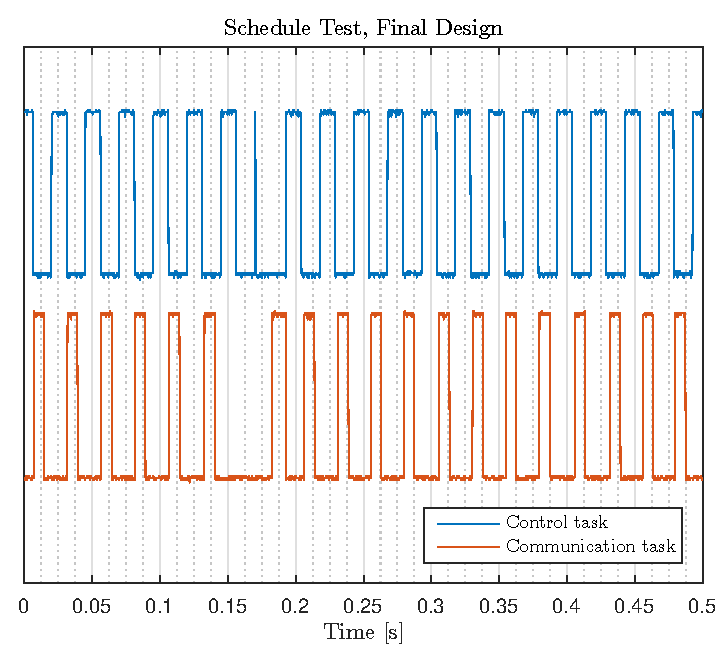
\includegraphics[width=1\linewidth]{figures/scheduleTestNew}
    \end{figure}                    
  \end{minipage}
\end{frame}
    
%%
% TOC
\begin{frame}{Agenda}{}
    \tableofcontents
\end{frame}

%%